\documentclass[a4paper, 11pt]{article}
\usepackage{comment} 
\usepackage{fullpage}
\usepackage{amsmath} 
\usepackage{amssymb} 
\usepackage{mathtools}
\usepackage{siunitx}
\usepackage{xfrac}
\usepackage{icomma}
\usepackage[section,below]{placeins}
\usepackage[labelfont=bf,font=small,width=0.9\textwidth]{caption}
\usepackage{subcaption}
\usepackage{graphicx}
\usepackage{grffile}
\usepackage{float}
\floatplacement{figure}{htbp}
\floatplacement{table}{htbp}
\usepackage{booktabs}
\usepackage{hyperref}
\sisetup{separate-uncertainty=true}

\begin{document}
\noindent
\centerline{\small{\textsc{Michigan State University}}} \\
\large{\textbf{CMSE/CSE 822 – Parallel Computing \hfill Fall 2019 \\
Homework 5}} \\
Alexander Harnisch \\
\noindent\makebox[\linewidth]{\rule{\textwidth}{0.4pt}}

The source files  \textit{codebreaker\_v2.c} and \textit{trapezoid\_hybrid.c}
\textbf{do not} exit in the instructor repository contrary to what you write in
the assignment, so it is a bit unclear where you want them.

\section*{1) MPI point-to-point vs collectives}
\subsection*{a)}
See code from repository.However, I have to make some comments here:
For debugging I added print sttements for the integral result in case the
result is wrong but forgot to set the brackets which leads to the value and
time printed twice if the result is correct. I realized this after my jobs were
already done and since HPCC is currently used heavily I did not want to restart
the jobs just because of redundant printing, the data is still correct.

Furthermore, the way I implemented it here makes rank 0 exclusively a master
communication process which does not perform any calculations itself. I adjust
for that by calling mpirun for one more process than required for the current
run. Also something that I would do differently (and have for the bonus part),
but since it does not effect the result at all I don't see a reason to change
it.

\FloatBarrier
\subsection*{b)}
The implementation has been timed for various numbers of sampling points (n =
1000, 100000 and 10M) and MPI processes (p = 1, 2, 5, 10, 20, 100, 250). Using
this data, the speed-up and efficiency for every data point was computed. The
results can be seen in Figure~\ref{fig:1_n_1000}, Figure~\ref{fig:1_n_100k} and
Figure~\ref{fig:1_n_10M}.

These plots have several features that can be easily understood: In all cases
(independent of the communication method used) the implementation does not
scale well with the number of used processes after a certain threshold. The
overhead produced by the parallelization is not worth it any more after that
threshold for $p$ has been reached. Where that threshold is depends on the
complexity of the problem.  For a higher complexity (larger $n$) the threshold
is also larger. This threshold can be clearly seen by a steep drop in
efficiency, which stays close to one before the threshold. 

It is also clear that The collective implementation generally clearly
outperforms the point-to-point implementation. However, that effect is a lot
stronger for larger values of $p$, which makes sense as the amount of required
communication is directly proportional to $p$. For small values of $p$ there is
almost no difference between the implementations.

\begin{figure}
  \centering
  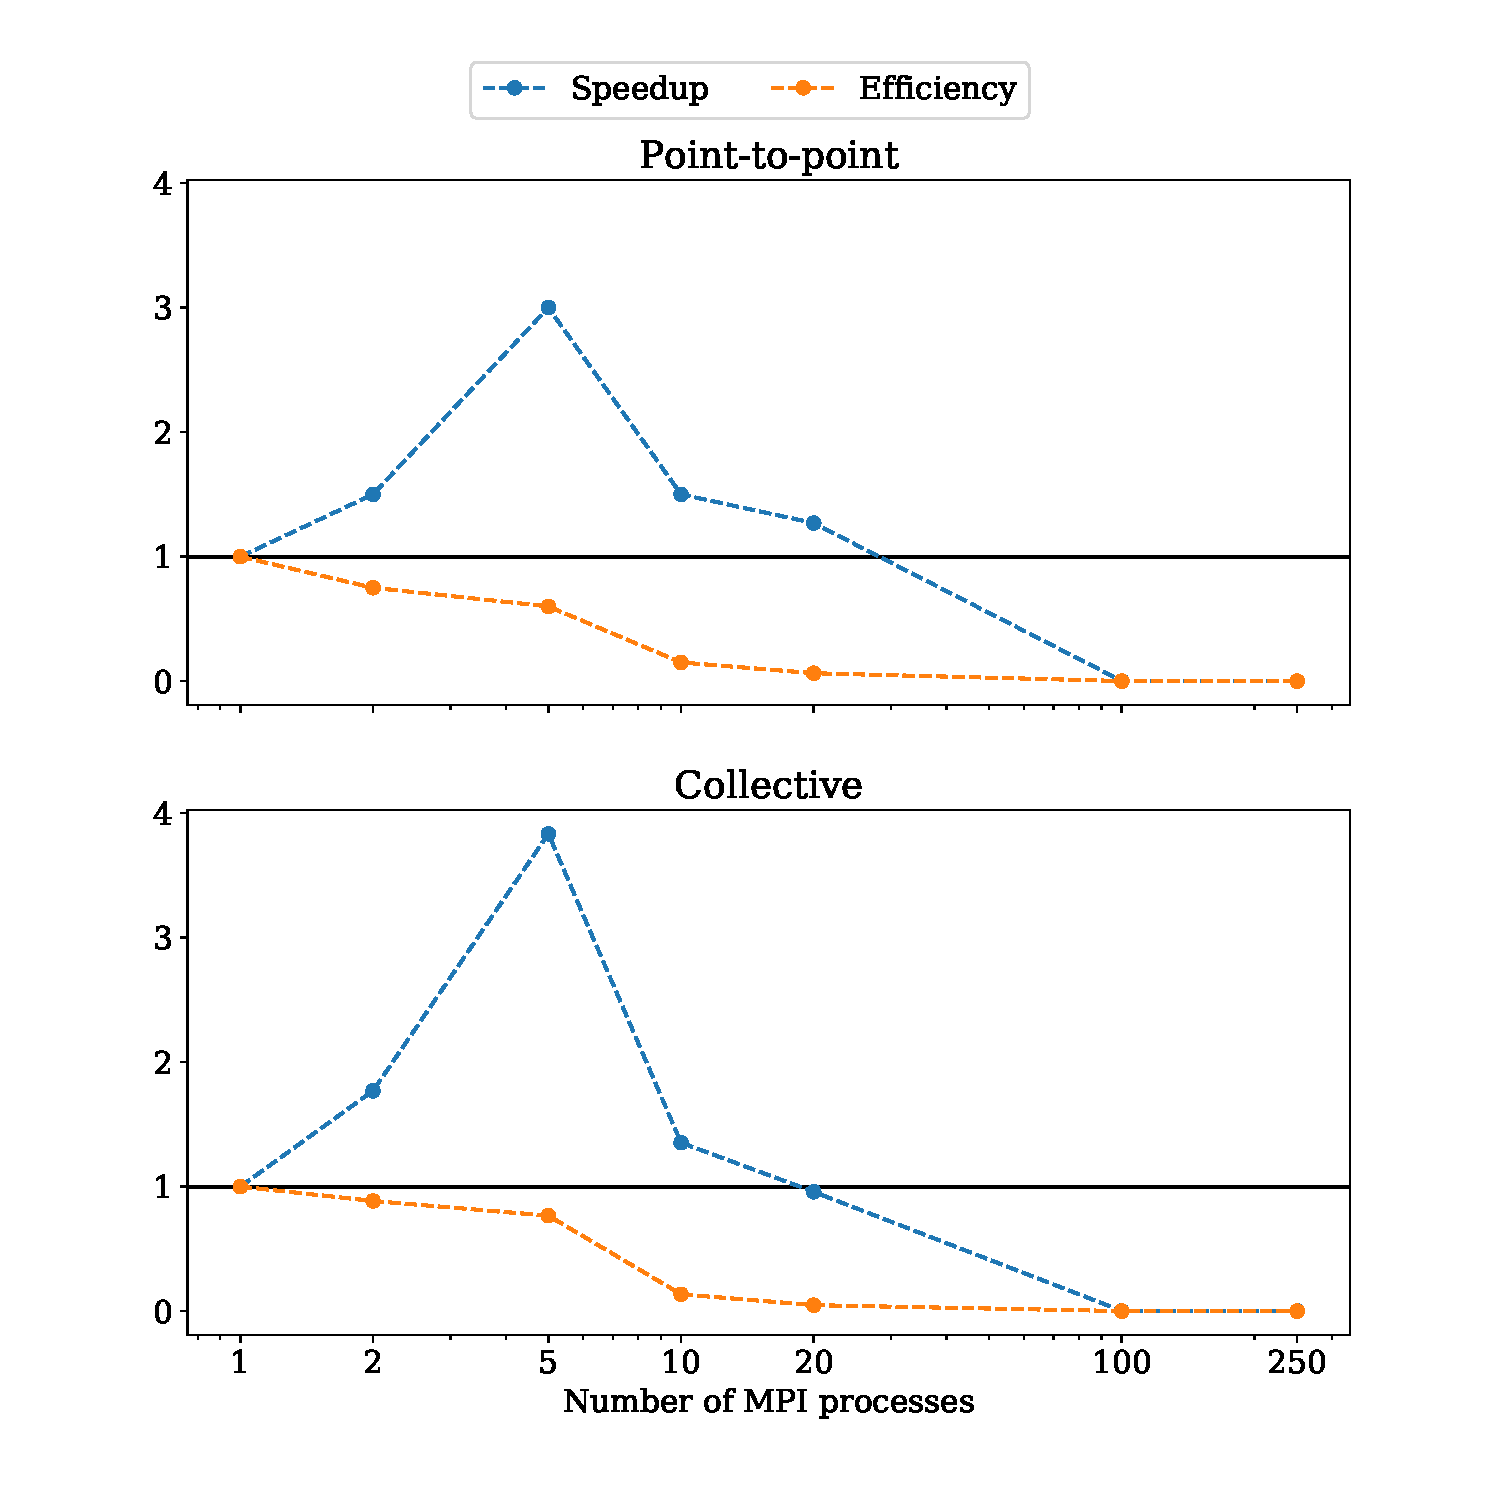
\includegraphics[width=\textwidth]{../trapezoid/plot/1000.pdf}
  \caption{Speedup and efficiency using point-to-point and collective communication for $n=1000$ sampling points.}
  \label{fig:1_n_1000}
\end{figure}
\begin{figure}
  \centering
  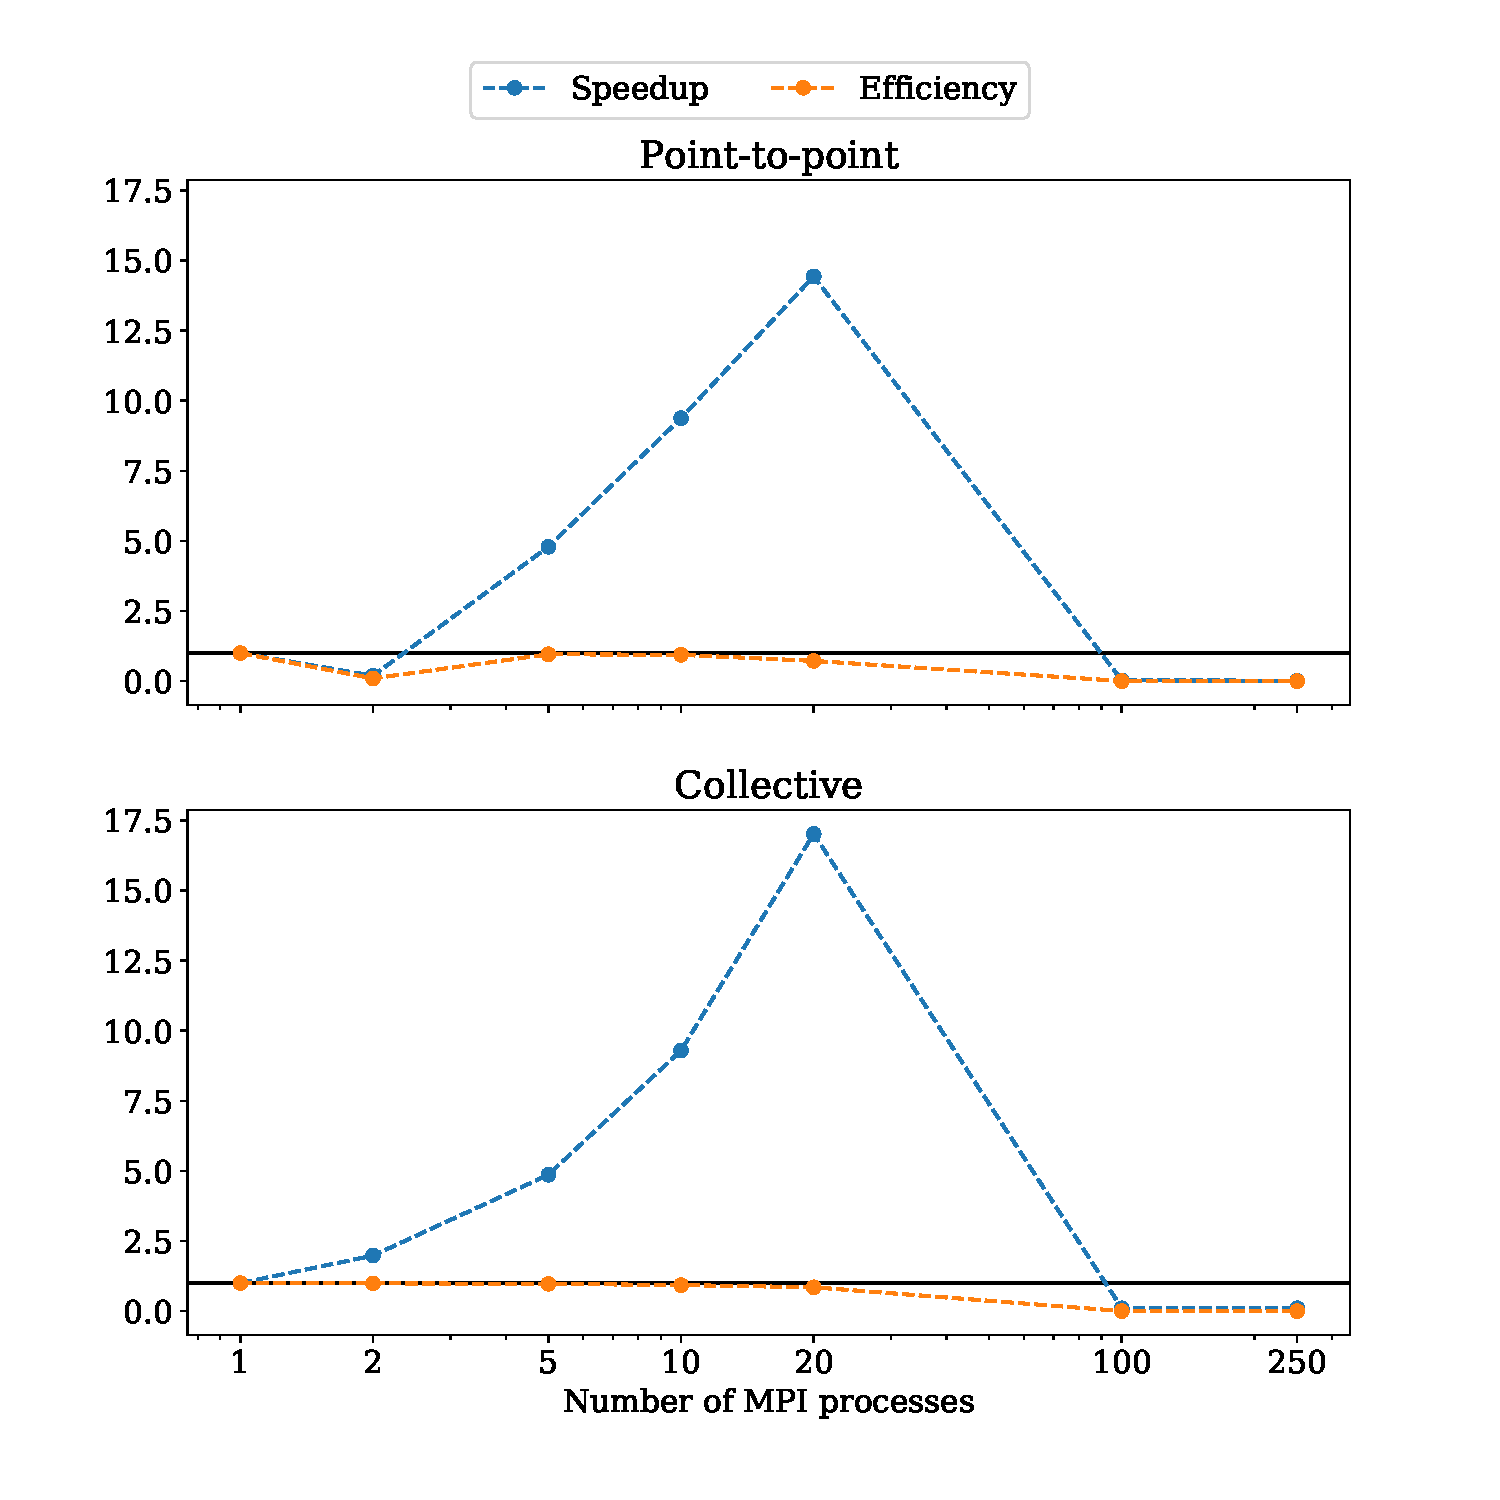
\includegraphics[width=\textwidth]{../trapezoid/plot/100000.pdf}
  \caption{Speedup and efficiency using point-to-point and collective communication for $n=10^{5}$ sampling points.}
  \label{fig:1_n_100k}
\end{figure}
\begin{figure}
  \centering
  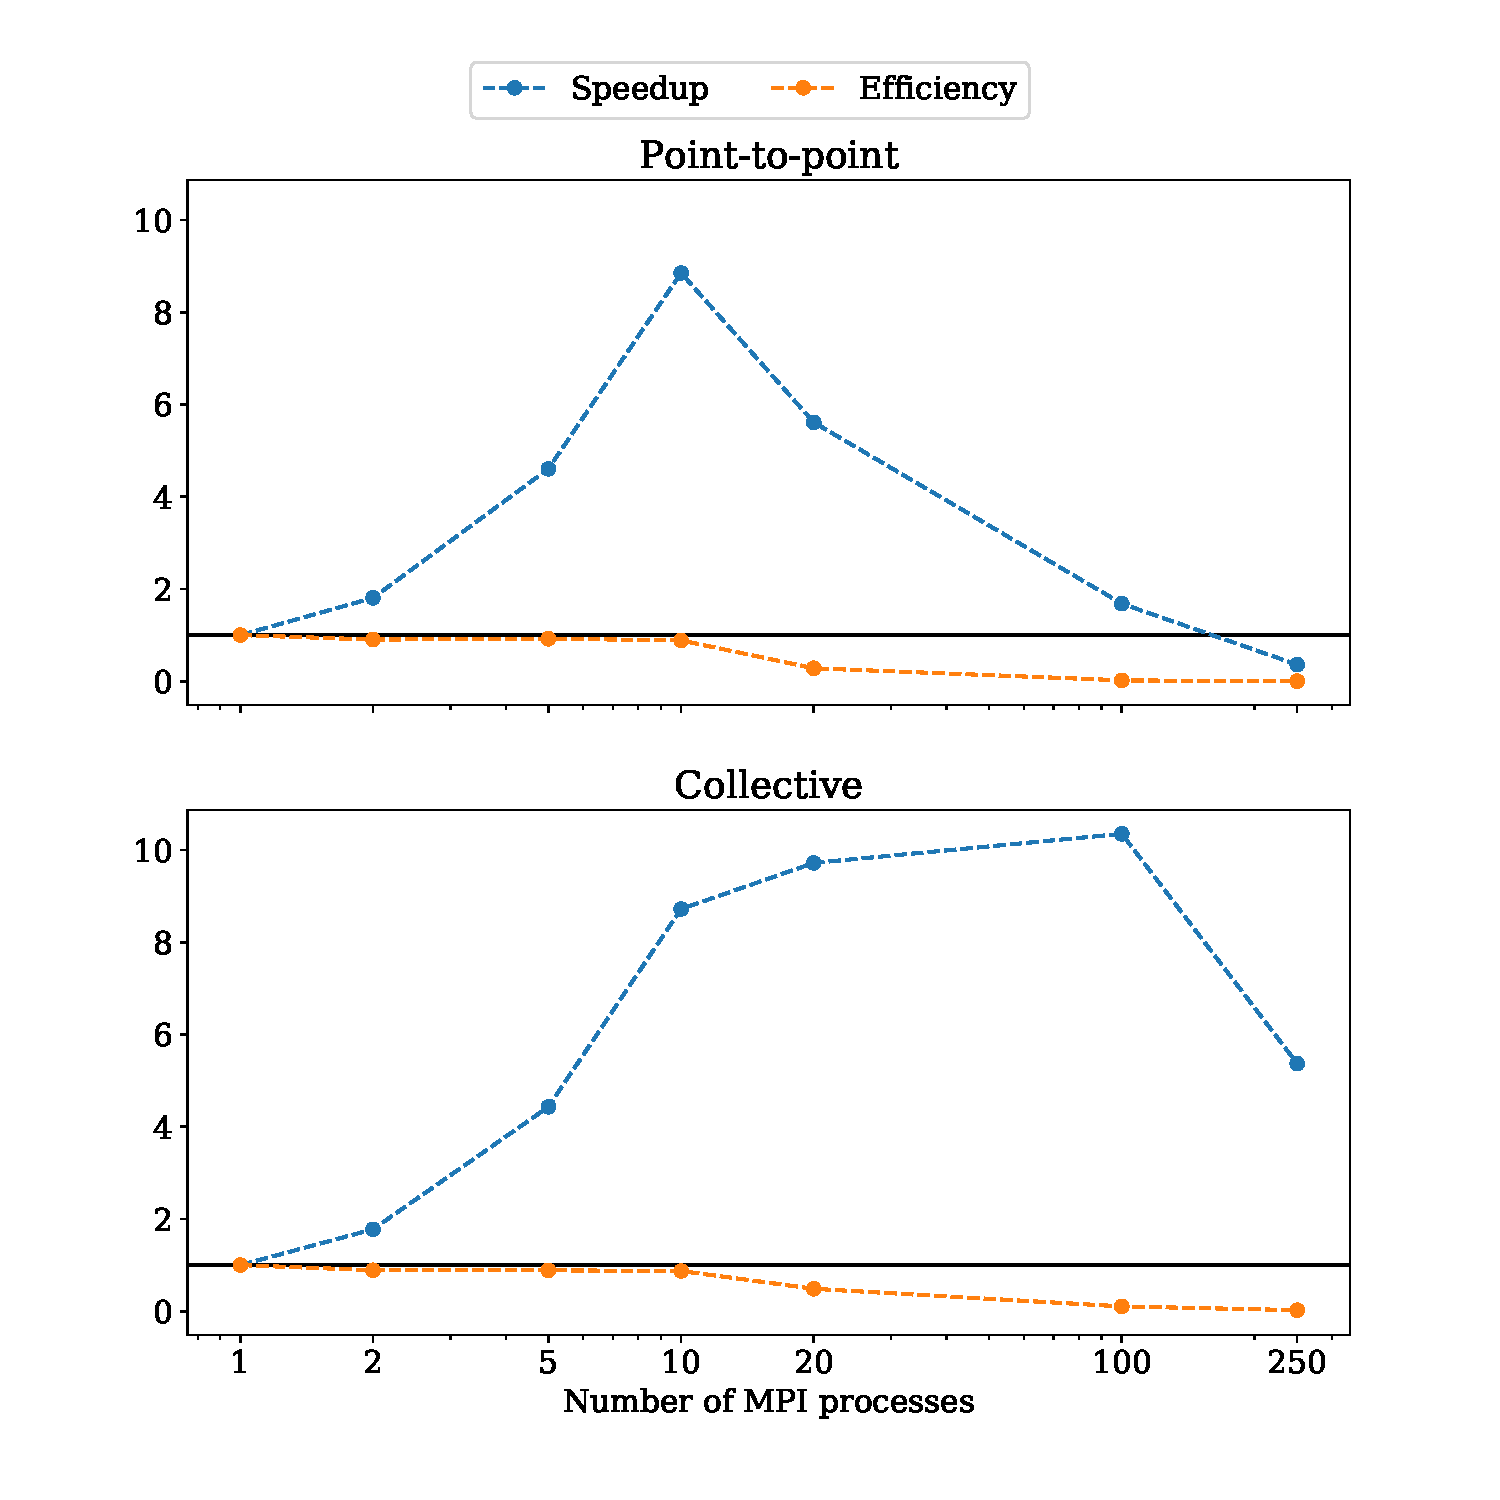
\includegraphics[width=\textwidth]{../trapezoid/plot/10000000.pdf}
  \caption{Speedup and efficiency using point-to-point and collective communication for $n=10^{7}$ sampling points.}
  \label{fig:1_n_10M}
\end{figure}

\FloatBarrier
\subsection*{c)}
The fitted parameters are listed in Table~\ref{tab:fit_paras}. The
corresponding fit results are visualized by Figure~\ref{fig:fit_1000},
Figure~\ref{fig:fit_100k} and Figure~\ref{fig:fit_10M}. The fitted model does
not take overhead into account. For that reason it is neccessary to exclude
data points that can not be described by the model. So for all fits only data
points have been used up until to the first value where the speed-up dropped
(see Figures in last subsection). In that range the model fits the data with
high accuracy, as can be seen in the figures and by looking at the small
standard deviations of the fitted parameters in Table~\ref{tab:fit_paras}.
 
\begin{figure}
  \centering
  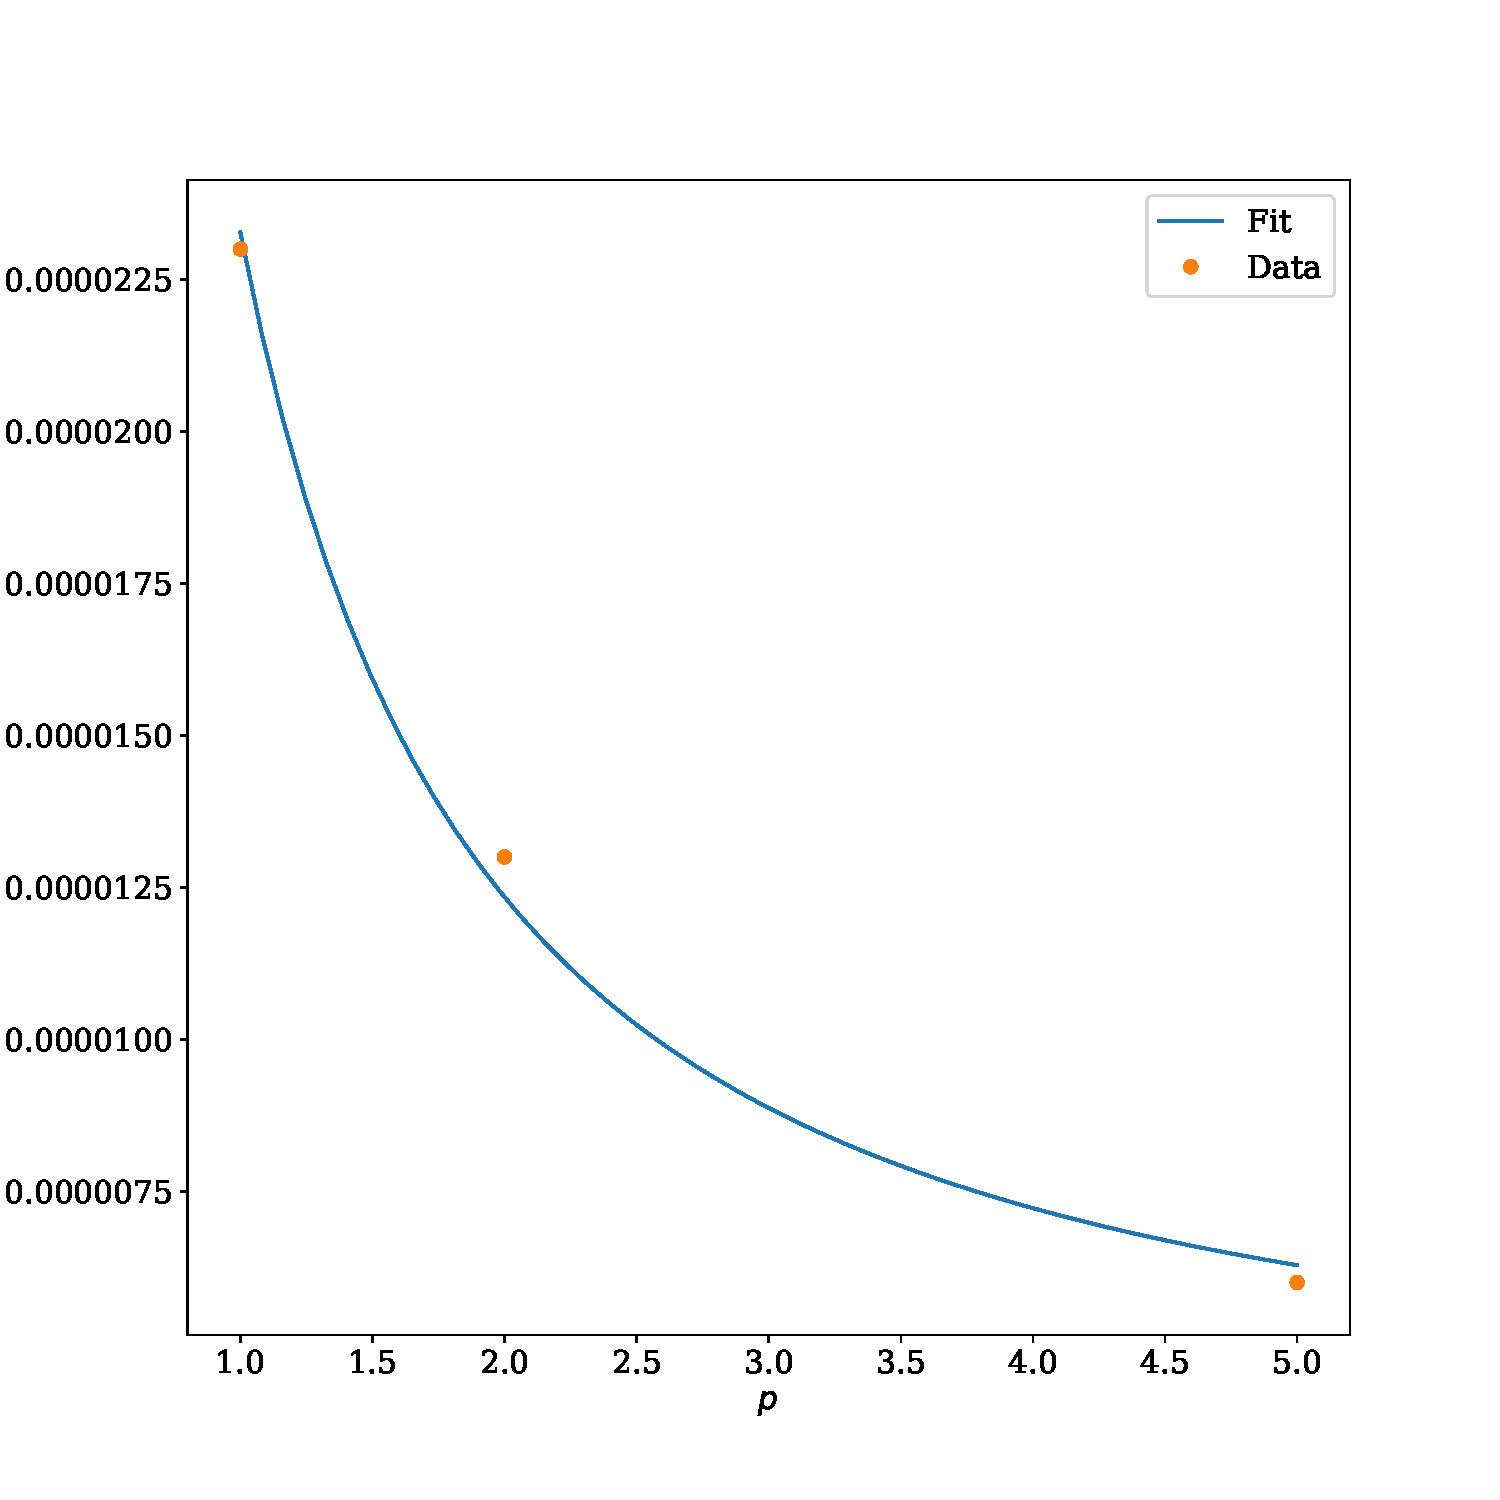
\includegraphics[width=\textwidth]{../trapezoid/plot/fit_1000.pdf}
  \caption{Least square fit for $n=1000$.}
  \label{fig:fit_1000}
\end{figure}
\begin{figure}
  \centering
  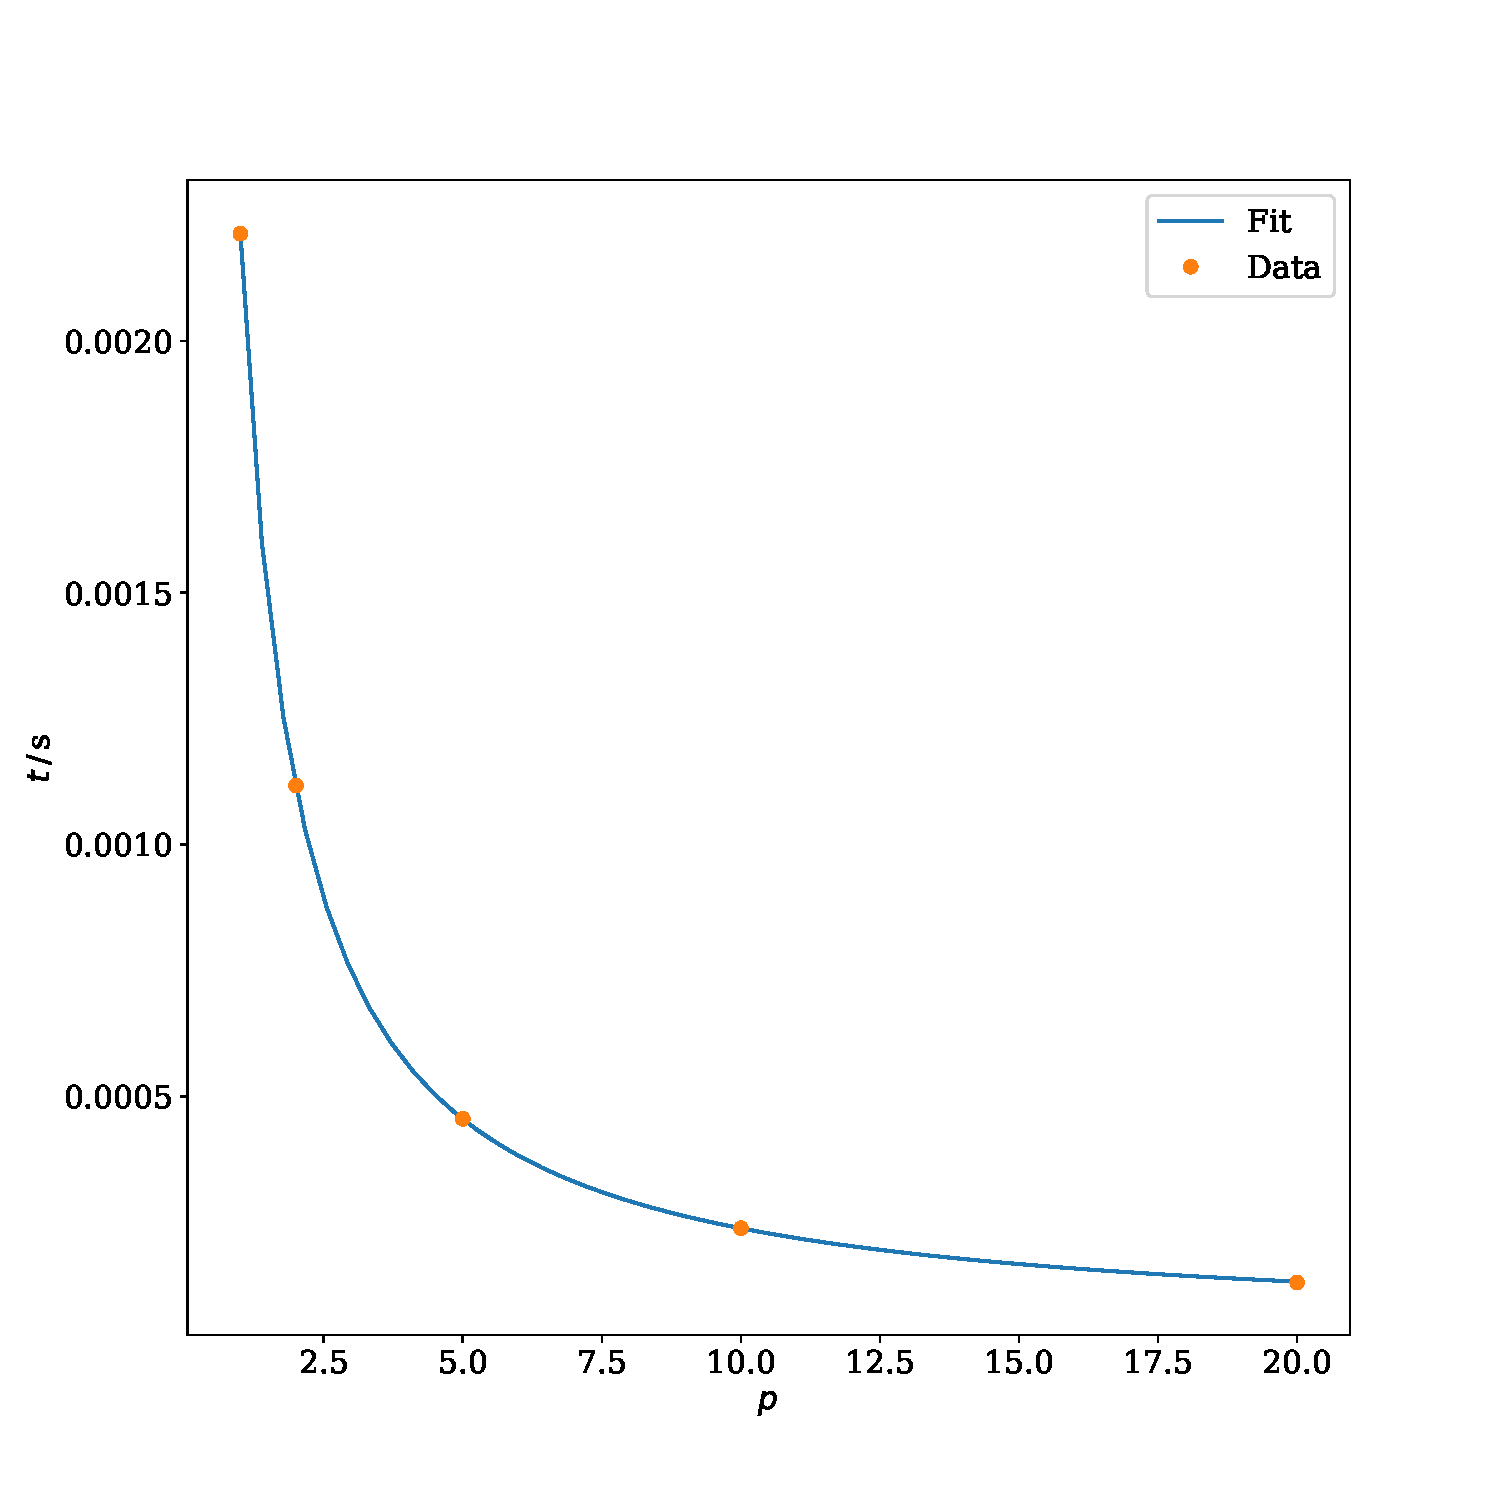
\includegraphics[width=\textwidth]{../trapezoid/plot/fit_100000.pdf}
  \caption{Least square fit for $n=10^{5}$.}
  \label{fig:fit_100k}
\end{figure}
\begin{figure}
  \centering
  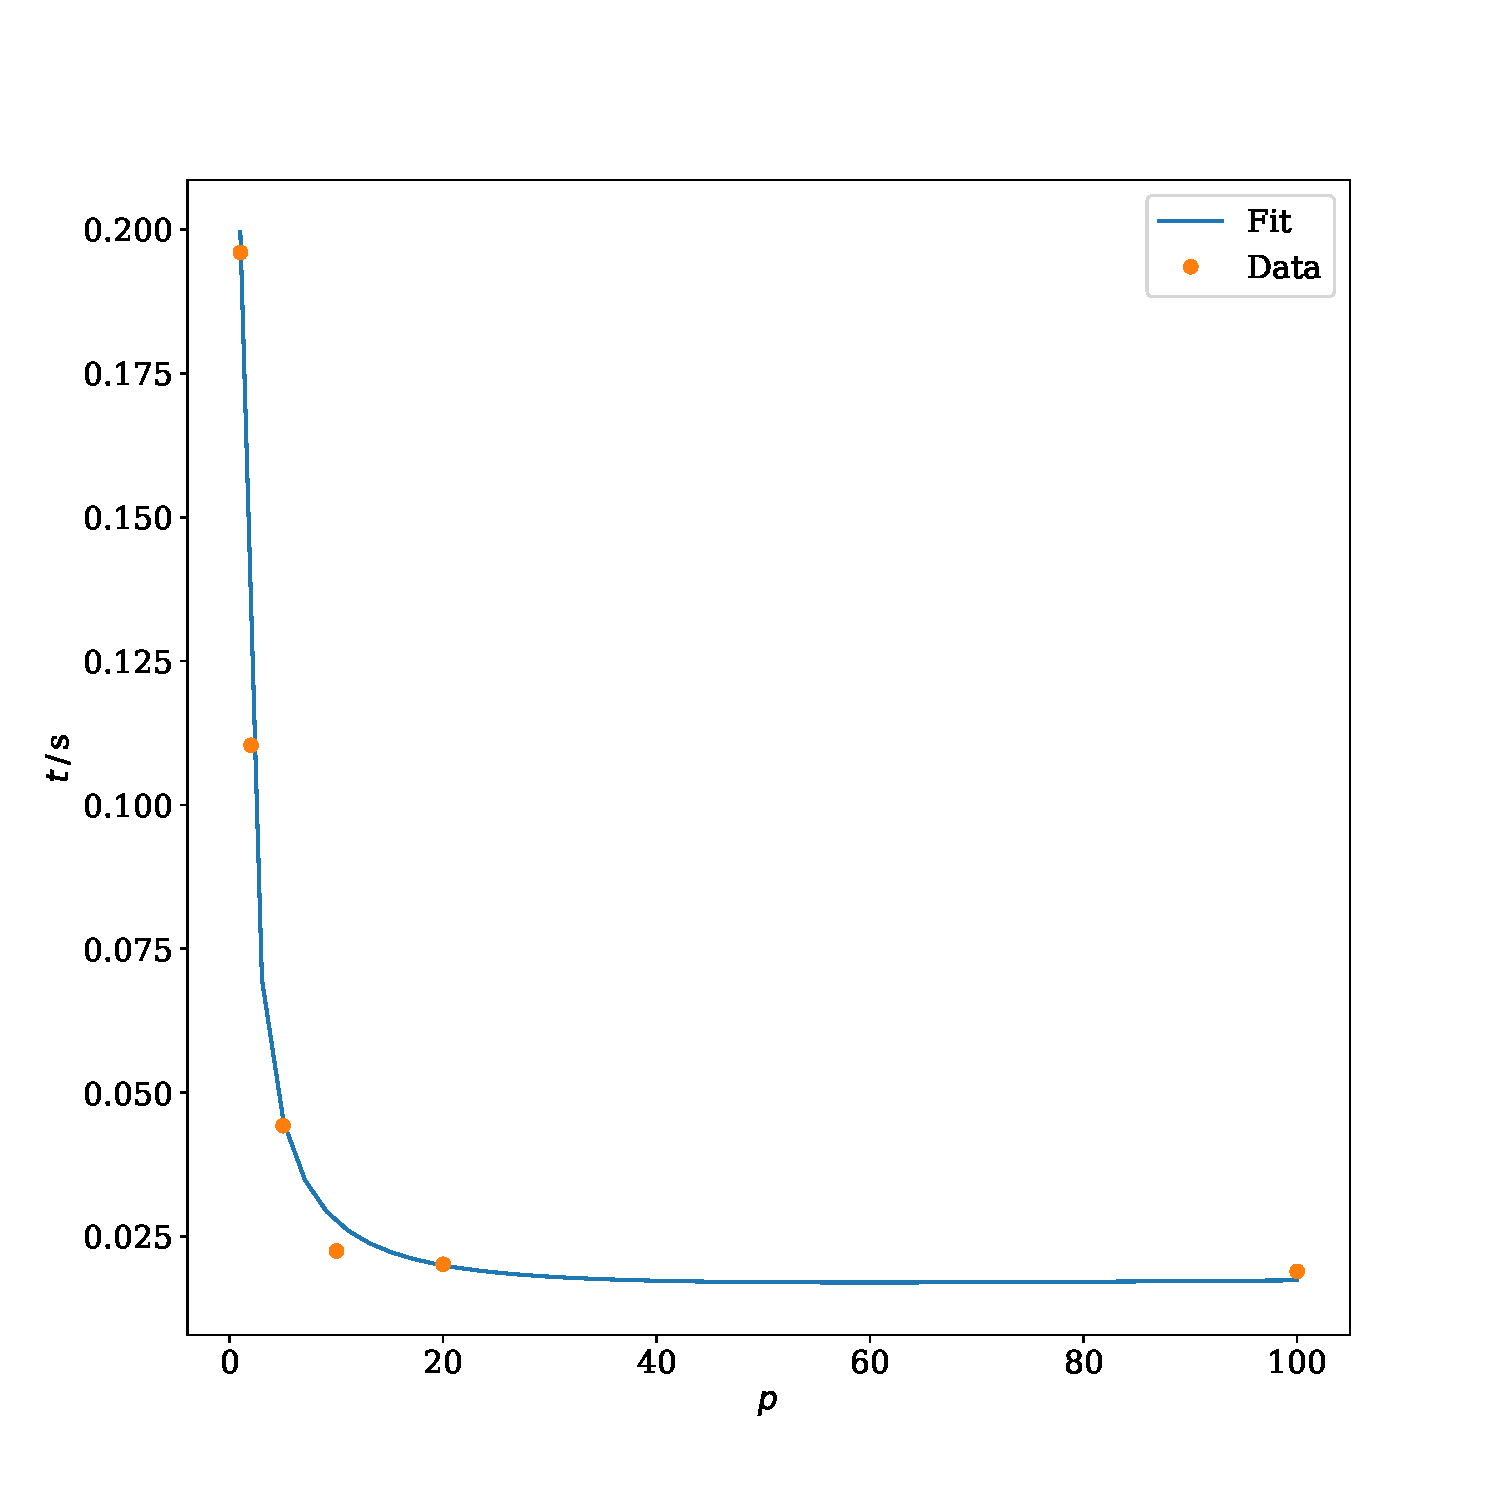
\includegraphics[width=\textwidth]{../trapezoid/plot/fit_10000000.pdf}
  \caption{Least square fit for $n=10^{7}$.}
  \label{fig:fit_10M}
\end{figure}
\begin{table}[ht]
\small
\begin{tabular}{lll}
$n$      & a / s                                          & b / s                 \\
\hline
$10^{3}$ & 2.327363481111708e-08 $\pm$ 7.198806692920759e-10 & 7.020128452971986e-07 $\pm$ 3.234141860026084e-07 \\
$10^{5}$ & 2.2153350279079064e-08 $\pm$ 2.7982074194404577e-11 & 4.843159937388218e-06 $\pm$ 5.3147319516767e-07 \\
$10^{7}$ & 1.9949962301415306e-08 $\pm$ 4.67814210500844e-10 & 0.0023154202059335717 $\pm$ 0.0005960271517657326 \\
\end{tabular}
\caption{Fitted parameters for the runtime using collective communication.}
\label{tab:fit_paras}
\end{table}

\FloatBarrier
\subsection*{BONUS: MPI/OpenMP parallelization}
No time left to create plots. I did implement and test it though. I do not find
a performance increase at all in this case. Which I think is because OpenMPI
does use shared memory if possible and OpenMP pretty much only adds additional
overhead. 

\section*{2) Code Breaking}
\subsection*{a)}
See code in repository. 

The code for my cyclic implementation for part c) is
\textit{cyclic\_codebreaker.c} in the \textit{src} directory.

\subsection*{b) and c)}
Okay so I find this and the next part of the assignment a huge waist of
computational resources and rather pointless. The partitioning scheme is
completely irrelevant in practice, assuming the keys to crack are uniformly
distributed. No matter what the partitioning scheme is, one can always get
ultimately lucky (the key is the first to try by any process) or unlucky (the
key is the last to try in the partitioning scheme). 

In any case (except for random partitioning), the runtime is always
pre-determined and only dependent on the partitioning scheme, number of
processes, \textbf{the time it takes to test one specific key} and the key
itself.

However, in case the key is not drawn from a uniform distribution and the
distribution it is drawn from is known (or we have a good guess), the most
efficient partitioning scheme to use would obviously be a cyclic scheme
iterating over a list of all keys which is sorted by each key's probability in
the distribution. For example, if we know the key is actually chosen by a human
we know that humans strongly prefer to choose the digits 3 and 7 over all
others, so we would want to try keys that have 3s and 7s in them first and
cycle over them in all threads. Same with some letters/words, you get what I
mean. But since the assignment does not specify at all from what distribution
the keys are chose, \textbf{there is no way to overcome what you call pitfalls
in c) in the general case}.

Of course I can choose the worst possible keys for block partitioning and then,
using that prior knowledge, find another partitioning scheme for which those
keys are the first to try. In fact, the optimal solution to c) would be
simply to hardcode all the examples I chose for b) and try those first. But I
have a feeling you wouldn't give me any points for that because I know what you
probably want is a cyclic scheme and that's what I have implemented for c)
because I don't feel like arguing over points haha. But I hope you get the
point I am trying to make here. \textbf{The point is: For actual practical
  purposes to crack a message that has been encrypted using a key drawn from a
  uniform distribution, the partitioning scheme is completely irrelevant. On
average, block partitioning and cyclic partitioning or whatever partitioning
will all perform equally.}

So back to the actual assignment, I don't feel like wasting a ton of HPCC
resources, so I will simply confirm my theoretical runtime prediction by
testing a few keys, which is what I think you want us to do here anyways.

The runtime is simple to predict: After applying the partitioning scheme we
have a list of keys that is tested by each process. The runtime is simply
the position of the actual key in the list it is on times the time it takes to
try a single key.

For the block partitioning scheme things are even simpler because the lists are
just ascending blocks and the positions are differences of keys on the list, so
the total runtime $T$ for any given key $k$ using block partitioning with $p$
processes and a total allowed range for the key between $0$ and
$k_{\textup{max}} - 1$ and a single-key-test-time (the time it takes one process to
test one key) of $\tau$ is:
\begin{equation}
  T = (k\mod\frac{k_{\textup{max}}}{p} + 1)\tau\,.
  \label{eqn:block_prediciton}
\end{equation}
However, this expression is only exact for $k_\textup{max}$ being a whole
multiple of $p$, generally the fracture has to be replaced by an integer
division and the last block is a little larger than all the others (just the
way I have implemented it).

So obviously the longest runtime (what you call zero speedup) would be
accomplished for any key that is at the end of a block. Technically it would
only be a speedup of zero if it is the last key in the first block, in which
case the sequential and parallel versions have the same runtime except for
overhead produced by the MPI stuff. What key that is obviously depends on $p$,
it is simply
\begin{equation}
  k_{\textup{max}}\div p\,,
\end{equation}
where I use $\div$ to annotate integer division. 

Obviously the key $k_{\textup{max}} - 1$ will always result in the longest
runtime no matter what $p$ is and the speedup will be (almost) linear. I really
think it doesn't make a lot of sense to talk about speedup for specific keys
here. When talking about speedups the average case should be considered,
otherwise we are just talking about worst and best case scenarios. As mentioned
earlier, the average speedup for uniformly sampled keys will always be linear
no matter what the partitioning scheme is.

The only thing that actually makes sense to measure here is $\tau$. I did so
for all versions of the codebreaker (sequential, block partitioning and cyclic
partitioning in c)). Simply running the executable for a specific amount of
repetitions to time the loop provides us with an average and standard
deviation. On intel16 I get:
\begin{equation}
  \tau_\textup{sequential} = \SI{1.444 \pm 0.013}{\micro\second}\,,
  \label{eqn:tau_sequential}
\end{equation}
\begin{equation}
  \tau_\textup{block} = \SI{1.605 \pm 0.012}{\micro\second}\,
  \label{eqn:tau_block}
\end{equation}
and
\begin{equation}
  \tau_\textup{cycllic} =\SI{1.554 \pm 0.015}{\micro\second}\,.
  \label{eqn:tau_cyclic}
\end{equation}

It makes sense, that we get the lowest average and standard deviation of $\tau$
for the sequential version, since it has no overhead and variance through
communication times. It also makes sense, that we get roughly the same time and
standard deviation for block and cyclic partitioning since the only difference
is the conditional statement in the for loop for the cyclic implementation to
test if the current iteration should be skipped, which luckily does not result
in a runtime penalty thanks to branch prediction.

It is also important to mention that $\tau$ is highly dependent on the input
and dictionary, but will always be constant for the same input and dictionary.
The values I have tested here result from using your \textit{inp1.txt} file and
provided dictionary.

So using the measurement for $\tau_\textup{block}$ we can predict the runtime
for the blocked partitioning for any number of processes $p$ using
\eqref{eqn:block_prediciton}. Sadly it is already 5 pm and I only have time until midnight, so I won't be able to test the worst case for small $p$'s. The worst case for sequential execution would take
\begin{equation}
  \small
  T_\textup{worst}(p = 1) = k_\textup{max} \tau_\textup{sequential} = 2^{32}\cdot\SI{1.595 \pm 0.005}{\micro\second} = \SI{6851 \pm 20}{\second}\, = \SI{1.903 \pm 0.006}{\hour}.
\end{equation}

Okay I guess I could still start jobs for that, but it's such a waist to spend
2 CPU hours on that\dots

So I decided to just choose one example key for the three cases you describe
and test it for various $p$ and plot that together with my prediction, which
should be very accurate. 

So obviously the best choice for ``super-linear'' speedup would be the first
key in the last block. The runtime should therefore just be
$\tau_\textup{block}$, except for the fact that especially the first execution
of the loop will probably take a little longer than that. So let's say we want
that for $p=14$ (using all physical cores on intel16 at once). The key
according to \eqref{eqn:block_prediciton} should be
\begin{equation}
  k_1 = 13\cdot (2^{32} \div 14) = 3988183917
  \label{eqn:k_1}
\end{equation}
resulting in a speedup of
\begin{equation}
  s = T(p = 1, k = k_1)/T(p = 14, k = k_1) = T(p = 1, k = k_1)/\tau_\textup{block} = (k_1 - 1)
\end{equation}
which is definitely more than 14 and therefore ``super-linear''!

The second key I choose is the ``linear speedup'' one. Those keys are the ones
that are at the end of the block. Actually it would only be the one at the end
of the last block and in the case where the block size is a whole multiple of
the maximum key. However, my formula breaks in that point because it does not
take into account that my last block is a little bigger than all the others to
make up for block size not being a whole multiple of the maximum key. Therefore
I simply choose the key to demonstrate linear speedup to be the highest where
the largest where the formula doesn't break, which is  
\begin{equation}
  k_2 = k_\textup{max} - 23 = 4294967273\,.
\end{equation}
For the ````no speedup'' scenario the obvious choice is the last key in the
first block (but it can be any key in the first block). So for $p = 14$ that's
\begin{equation}
  k_3 = (2^{32} \div 14) - 1
\end{equation}

So at this point I only have 2 hours until the deadline left, so I can't really
test that many values sadly. However, to proof my point, it is totally
unnecessary to measure any combinations anyways, as they perfectly fit my
prediction. My results for the blocked partition can be seen in
Figure~\ref{fig:block}.

\begin{figure}
  \centering
  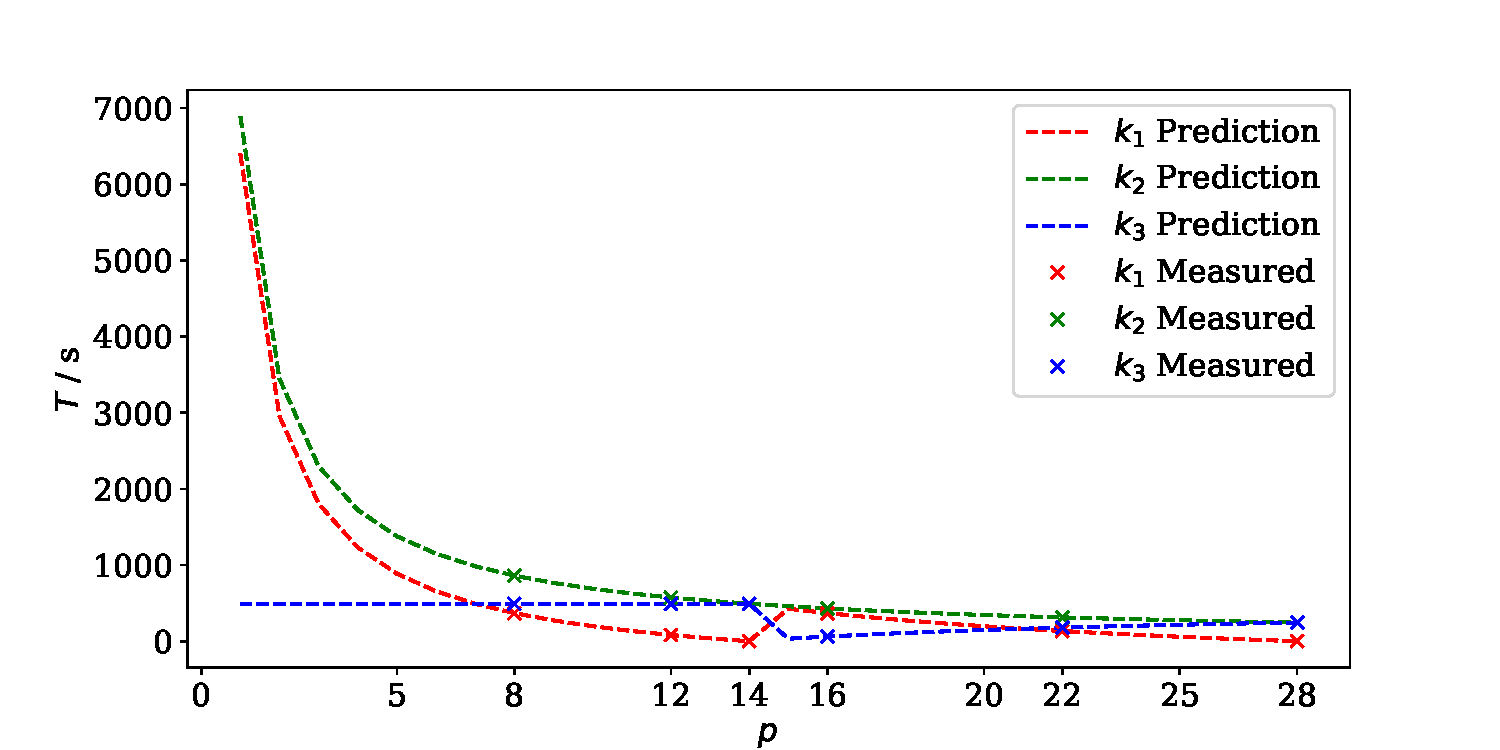
\includegraphics[width=\textwidth]{../codebreaker/plot/block.pdf}
  \caption{Prediction and measurements for blocked partitioning.}
  \label{fig:block}
\end{figure}

Definitly don't have enough time to give the analytical formula to predict the
same thing for cyclic partitioning, but Figure~\ref{fig:cyclic} shows the
measured values. As required by the assignment, the ````pitfall'' is avoided.
However, it's an illusion as discussed earlier. Sorry I would plot it nicer to
make it more easily comparable but I really don't have the time.

\begin{figure}
  \centering
  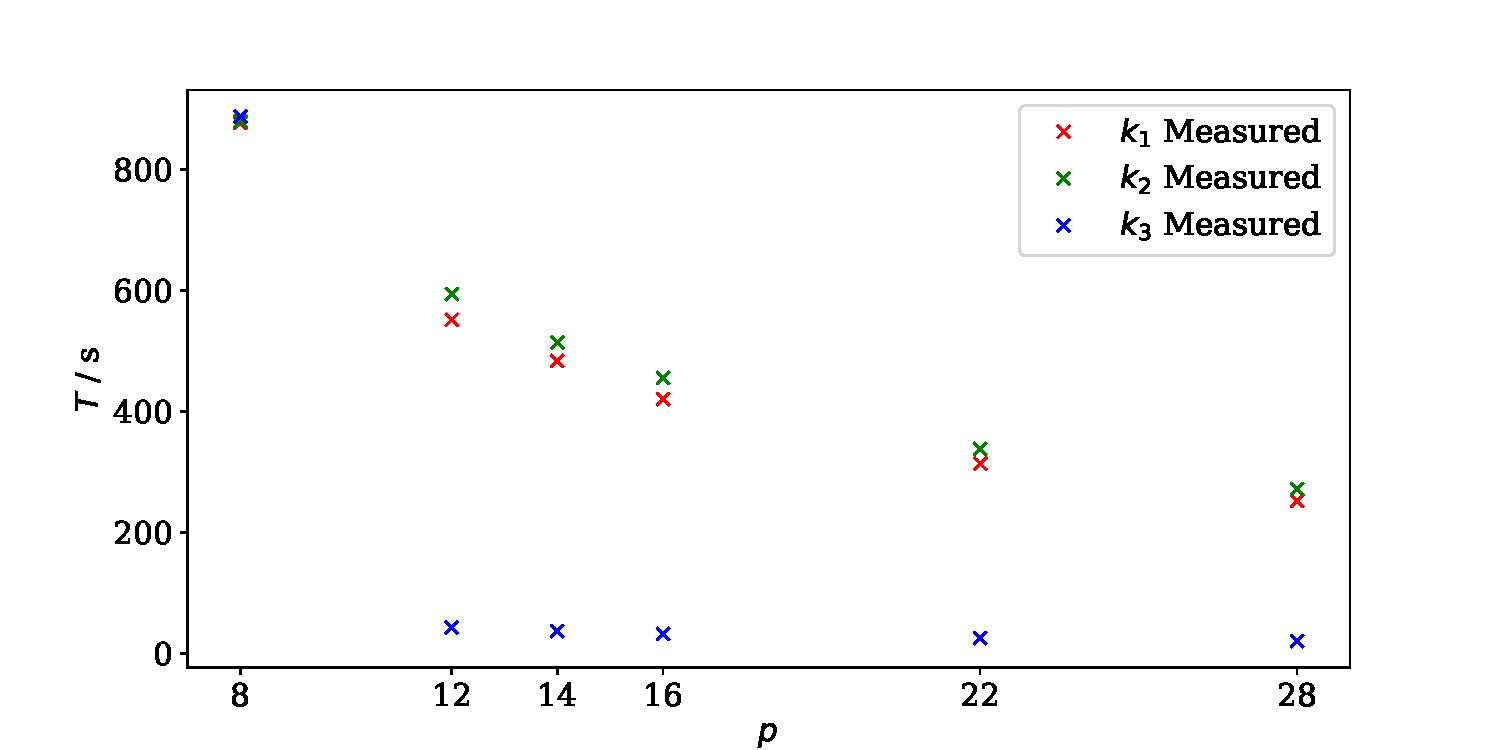
\includegraphics[width=\textwidth]{../codebreaker/plot/cyclic.pdf}
  \caption{Measurements for cyclic partitioning.}
  \label{fig:cyclic}
\end{figure}

\end{document}
